\documentclass[a4paper,12pt]{article}
\usepackage{fancyhdr}
\usepackage{lastpage}
\usepackage{geometry}
\usepackage{listings}
\usepackage{datetime}
\usepackage{xeCJK}
\usepackage{hyperref}
\usepackage{amsmath}
\usepackage{graphicx}
\usepackage{float} % 加入 float 宏包以使用 [H]
\usepackage{longtable}

\geometry{left=2.5cm, right=2.5cm, top=2.5cm, bottom=2.5cm}
\pagestyle{fancy}
\setCJKmainfont{Noto Sans CJK HK}
% 英文字體 consolas
\setmonofont{Consolas}
% 設定內文文字大小
\renewcommand{\normalsize}{\fontsize{12pt}{\baselineskip}\selectfont}

% 設定頁首
\fancyhf{}
\fancyhead[L]{ISO Surface Visualization}
\fancyhead[R]{\today}
\fancyfoot[C]{\thepage/\pageref{LastPage}}

\title{ISO Surface Visualization}
\author{01057033洪銘均}
\date{\today}

\begin{document}
\maketitle
\tableofcontents
\newpage

\section{程式概述}
這個程式的主要功能是使用OpenGL來實現ISO Surface的可視化,並且使用Marching Cubes演算法來生成ISO Surface。程式中包含了讀取RAW檔案、計算ISO Surface、以及將結果渲染到螢幕上的功能。

\section{檔案與功能}
以下是每個原始碼檔案的簡要描述:
\begin{itemize}
    \item \texttt{main.cpp}:主程式,負責初始化 OpenGL 環境、載入著色器、以及處理使用者輸入。
    \item \texttt{phong.frag}:片段著色器,負責計算每個像素的顏色。
    \item \texttt{phong.vert}:頂點著色器,負責將三維座標轉換為二維座標。
    \item \texttt{reader.h reader.cpp}:讀取RAW檔案。
    \item \texttt{iso\_surface.h iso\_surface.cpp}:實現ISO Surface的演算法。
    \item \texttt{MarchingCubesTables.hpp}:包含Marching Cubes演算法所需的查找表。
    \item \texttt{glsl.h}: 包含OpenGL著色器的相關函式。
\end{itemize}

\section{程式截圖}
\begin{figure}[H]
    \centering
    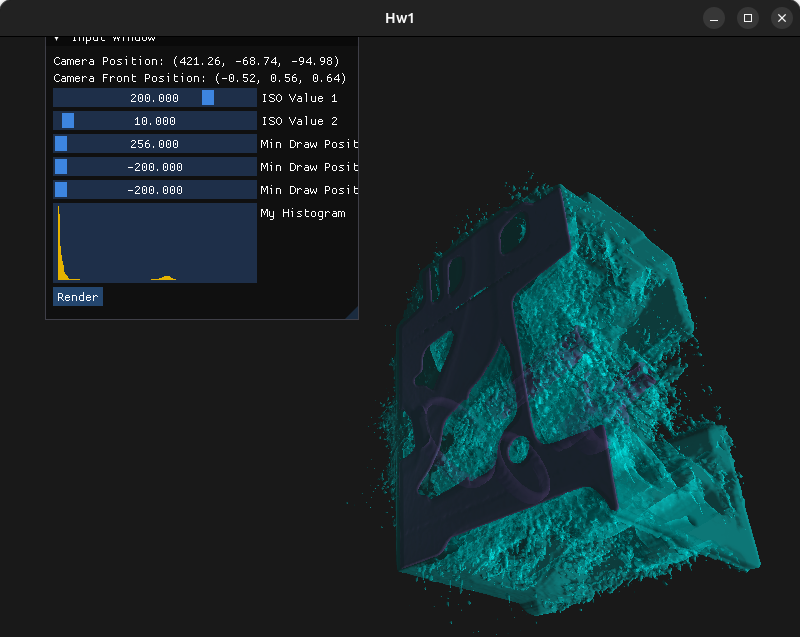
\includegraphics[width=0.8\textwidth]{img/img1.png}
    \caption{程式執行截圖}
    \label{fig:screenshot}
\end{figure}
\begin{itemize}
    \item 在UI中可以調整ISO值,最多可以調整兩層ISO值。
    \item 在UI中可以調整ISO Surface的切片,透過調整x, y, z要顯示的切片。
    \item 最底下的長條圖顯示ISO值的分佈情況,當ISO值越高時,顯示的長條圖會越高。
\end{itemize}

\section{心得}
這次的作業讓我學會了如何使用OpenGL來實現ISO Surface的可視化,並且了解了Marching Cubes演算法的基本原理。雖然在實作過程中遇到了一些困難,在最初一開始並非使用Marching Cube,而是使用Marching Tetrahedra,我手動計算了每個Cube中頂點對應在Tetrahedra中的位置,但生成出來的Vertex結果不正確,修改兩三天結果依舊,直到我改成使用Marching Cubes才正常,後續也檢查了Marching Tetrahedra的Table依舊找不到錯誤,也放棄了這個方法。\\
目前這程式功能已經算完整了,接下來會想要加入一些功能,例如:\textbf{1.}加入不同的顏色,\textbf{2.}更多層的ISO surface\textbf{3.}加速ISO Surface演算法。\\
\end{document}

% xelatex  --max-print-line=10000 -synctex=1 -interaction=nonstopmode -file-line-error -recorder .\codebook.tex 
